\documentclass[tikz,border=4pt]{standalone}
% Shared setup for the foundation-model diagrams, in the AFRICAST palette
\usepackage{fontspec}
\usepackage[sfdefault]{FiraSans}
\usepackage{amsmath}
\usepackage{unicode-math}
\setmathfont{Fira Math}
\usetikzlibrary{arrows.meta}
\definecolor{ink}{HTML}{1F2A36}
\definecolor{MonashBlue}{HTML}{3B75AC}
\definecolor{Orange}{HTML}{B5570F}
\color{ink}
\tikzset{every picture/.style={draw=ink,>=stealth}}
\hyphenpenalty=10000
\exhyphenpenalty=10000

\begin{document}
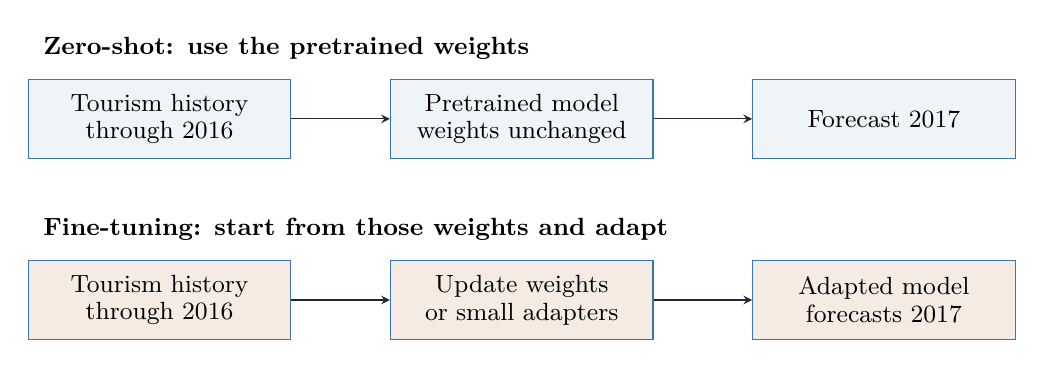
\begin{tikzpicture}[>=stealth,every node/.style={font=\fontsize{9}{10}\selectfont,align=center},
box/.style={draw=MonashBlue,fill=MonashBlue!8,text width=3.1cm,minimum height=1cm}]
\node[anchor=west,font=\fontsize{9}{10}\selectfont\bfseries] at (-1.6,.9) {Zero-shot: use the pretrained weights};
\node[box] (h1) at (0,0) {Tourism history\\through 2016};
\node[box] (m1) at (4.6,0) {Pretrained model\\weights unchanged};
\node[box] (f1) at (9.2,0) {Forecast 2017};
\draw[->] (h1)--(m1);\draw[->] (m1)--(f1);
\node[anchor=west,font=\fontsize{9}{10}\selectfont\bfseries] at (-1.6,-1.4) {Fine-tuning: start from those weights and adapt};
\node[box,fill=Orange!12] (h2) at (0,-2.3) {Tourism history\\through 2016};
\node[box,fill=Orange!12] (m2) at (4.6,-2.3) {Update weights\\or small adapters};
\node[box,fill=Orange!12] (f2) at (9.2,-2.3) {Adapted model\\forecasts 2017};
\draw[->] (h2)--(m2);\draw[->] (m2)--(f2);
\end{tikzpicture}
\end{document}
